\documentclass{beamer}
\usepackage{graphicx}
\usepackage{hyperref}
\usepackage{multimedia}
\usepackage{tikz}
\usepackage{bookman}
\usepackage{bookmark}
\usepackage{media9}
% \usetheme{Madrid}
\definecolor{ginger}{rgb}{0.69, 0.4, 0.0}
\usecolortheme{seahorse}
\title{Drop on Thin Film}
% \subtitle{}
\institute[IITD]{Indian Institute of Technology, Delhi}
\author{Kulwinder Kaur, Harikesh Kushwaha}
\begin{document}
\maketitle
\begin{frame}{Introduction}
    \frametitle{Introduction}
    \section{Introduction}
    \subsection{The Problem}
    \begin{enumerate}
        \item <1-> \textbf{The Problem}\\
              We are given a video of a drop leaving a needle and falling through a thin film. We are required to find the position of the drop in the film.
              \begin{center}
                  \movie[autostart, externalviewer]{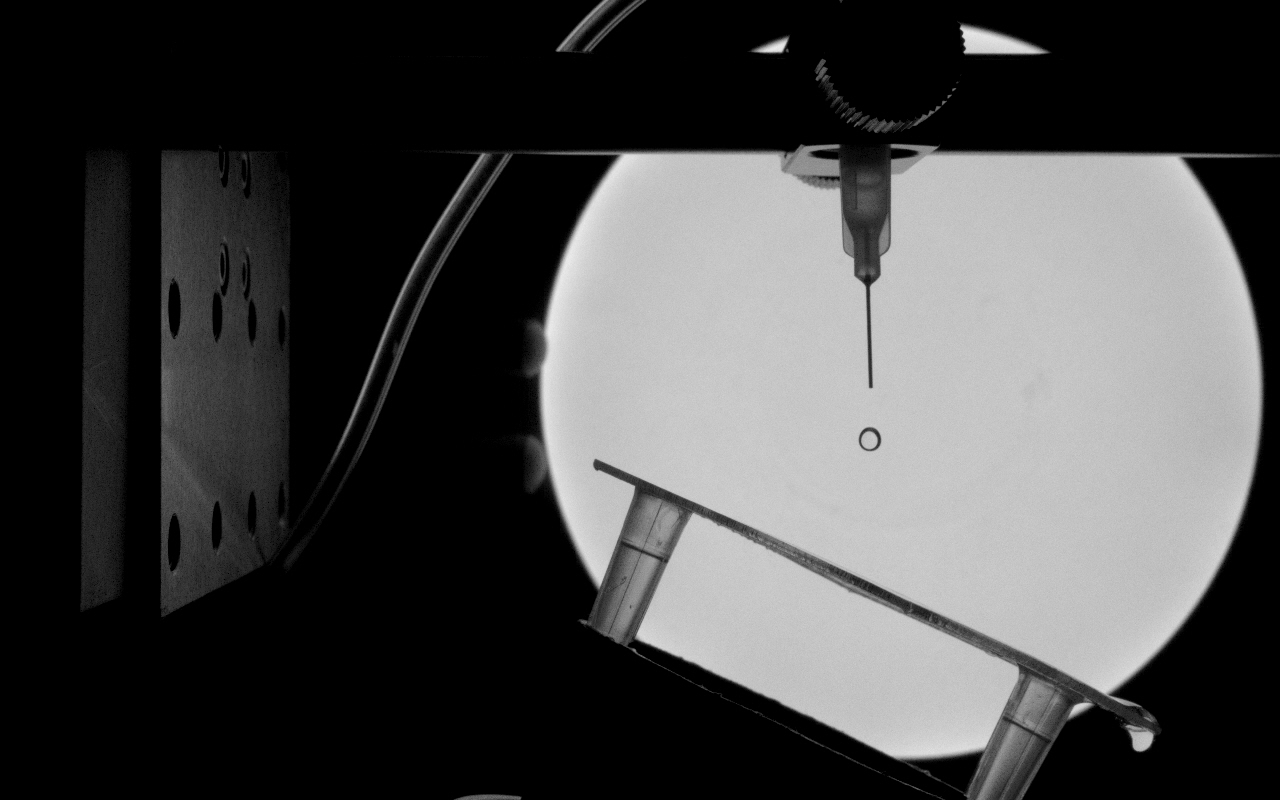
\includegraphics[scale=1.3]{34.jpg}}{drop_moving.mp4}
              \end{center}
              \subsection{Background Information}
        \item <2-> \textbf{Background Information}
              \begin{itemize}
                  \subsubsection{How Computer Stores Image?}
                  \item <2-> \textbf{How Computer Stores Image?}\\
                        Every image is made up of pixels. These pixels are stored in the form of an array with the shape \textcolor{blue}{[Height, Width, Colour Channel]}.Each of the pixels that represents an image stored inside a computer has a pixel value which describes how bright that pixel is, and/or what color it should be.
              \end{itemize}
    \end{enumerate}
\end{frame}
\begin{frame}{Background Information}
    \frametitle{Background Information}
    % \subsection{Background Information}
    \subsubsection{Various Type of Images}
    \begin{itemize}
        \item <1-> \textbf{Various Type of Images}\\
              Images can be classied into various types on the basis of how many colour channels they have. Some are:
              \begin{itemize}
                  \item <2-> Colour Image\\
                        Having 3 or 4 colour channels.
                  \item <3-> Greyscale Image\\
                        Having a single colour channel, hence the name grayscale.
                  \item <4-> Binary Image\\
                        Having a single colour channel. Also, the value of pixels are either 0 or 1.
              \end{itemize}
    \end{itemize}
\end{frame}
\begin{frame}{The Solution}
    \frametitle{The Solution}
    \section[]{The Solution}
    \subsection{Preprocessing}
    \begin{enumerate}
        \item <1-> \textbf{Preprocessing}\\
              Before we can try extracting the center of the drop, we need to do some preprocessing. Here are the steps:
              \begin{itemize}
                  \subsubsection[]{Loading Image}
                  \item <2-> \textbf{Loading The Original Image}\\ The image provided are grayscale in nature. We can use matplotlib or Pillow libraries to read them. This will give us a numpy array on which we can work.\subsubsection[]{Cropping The Image}
                  \item <3->\textbf{Cropping The Image}\\Only a small portion of the image is useful to us as the drop is remaining in a region which spans for just about \(500\times 500\) px. That's why we cropped the image to contain just this region.
              \end{itemize}
    \end{enumerate}
\end{frame}
\begin{frame}
    \frametitle{Preprocessing}
    \begin{figure}
        \centering
        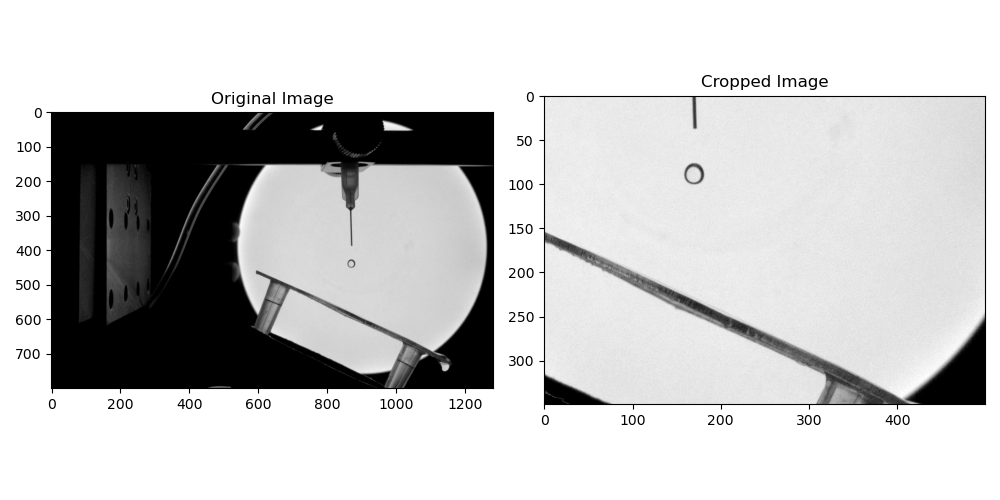
\includegraphics[scale=0.45]{cropped.png}
        \caption[]{Image Before and After Cropping}
    \end{figure}
\end{frame}
\begin{frame}
    \frametitle{Preprocessing}
    \subsubsection[]{Thresholding Image}
    \begin{itemize}
        \item <1-> \textbf{Thresholding Image}\\ Thresholding is the process of converting an image to a binary image. The thresholding is done by setting a certain value as the threshold. If the pixel value is greater than this threshold, it is set to 1, else it is set to 0.
    \end{itemize}
    \begin{figure}
        \centering
        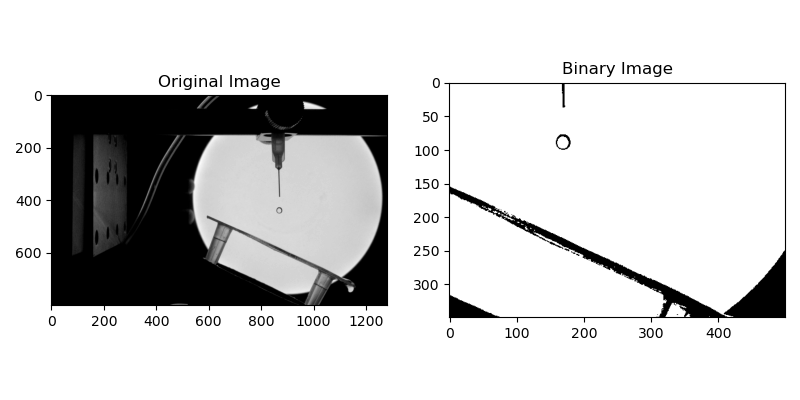
\includegraphics[scale=0.4]{binary.png}
        \caption[]{Image Before and After Cropping and Thresholding}
    \end{figure}
\end{frame}
\begin{frame}
    \frametitle{The Main Method}
    \section{The Main Method}
    \begin{figure}
        \centering
        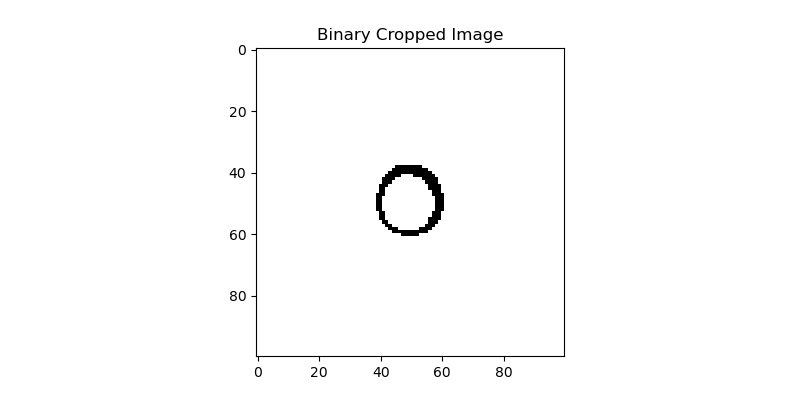
\includegraphics[scale=0.4]{small.png}
    \end{figure}
    The image above shows the drop with its surrounding restricted to just a 100 pixels. The image is a binary one, meaning that the pixel value is either 0 or 1. Zero for the black points and One for the white points. The idea behind the method we implemented to find the center of the drop is the following:
    \begin{itemize}
        \item <2-> Loop through the rows and find all the black pixels for each row.
    \end{itemize}
\end{frame}
\begin{frame}
    \frametitle{The Main Method}
    \subsection{Working of the Method}
    \begin{itemize}
        \item <1-> The position of the first such pixel will give the top-most point of the drop and the last such pixel will give the bottom-most point of the drop.
        \item <2-> Loop through the columnss and find all the black pixels for each columns.
        \item <3-> The position of the first such pixel will give the left-most point of the drop and the last such pixel will give the right-most point of the drop.
        \item <4-> Once we have the top-most, bottom-most, left-most and right-most points of the drop, we can find the center as well as the horizontal and vertical radii of the drop.
    \end{itemize}
\end{frame}
\begin{frame}
    \frametitle{The Main Method}
    \subsection{Working of the Method}
    Here is an animation showing the process of finding the center of the drop.\\
    \centering
    \movie[externalviewer, borderwidth=1pt]{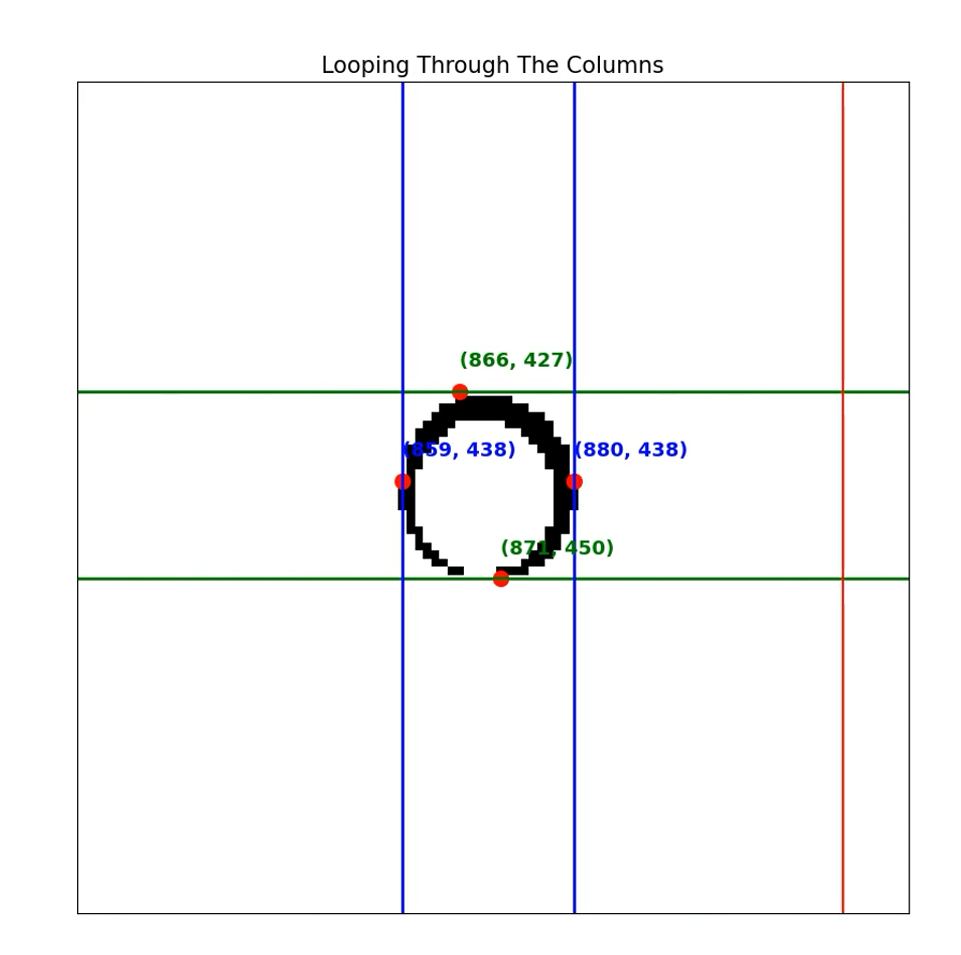
\includegraphics[scale=0.35]{method_poster.png}}{the_method.mp4}
\end{frame}
\begin{frame}
    \frametitle{Problems With The Main Method}
    \section{Problems With The Main Method}
    The method implemented above works fine for most cases but it does have some problems:
    \begin{itemize}
        \item <1-> When the drop is just leaving the needle and when the drop is leaving or near the edge of the film, the method fails.
              \begin{figure}
                  \centering
                  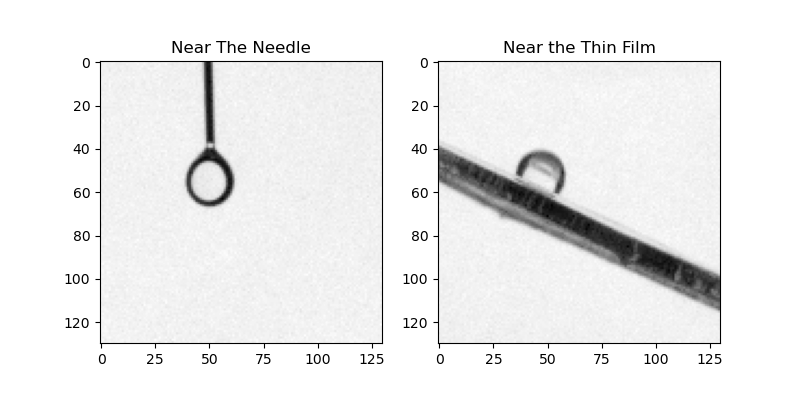
\includegraphics[scale=0.4]{problems1.png}
              \end{figure}
        \item <2-> We need to specify the crop coordiantes for each image. This leaves the method from being generic.
    \end{itemize}
\end{frame}
\begin{frame}
    \frametitle{Problems With The Main Method}
    \section{Problems With The Main Method}
    \small
    The second problem can be solved partially by using the dynamic cropping. In this method, we decide which portion of the image to crop on the basis of the center of the drop in previous image. We define a height and width and calculate the bounding box for the crop. Here is an animation showing the same.\\
    \centering
    \movie[externalviewer, borderwidth=1pt]{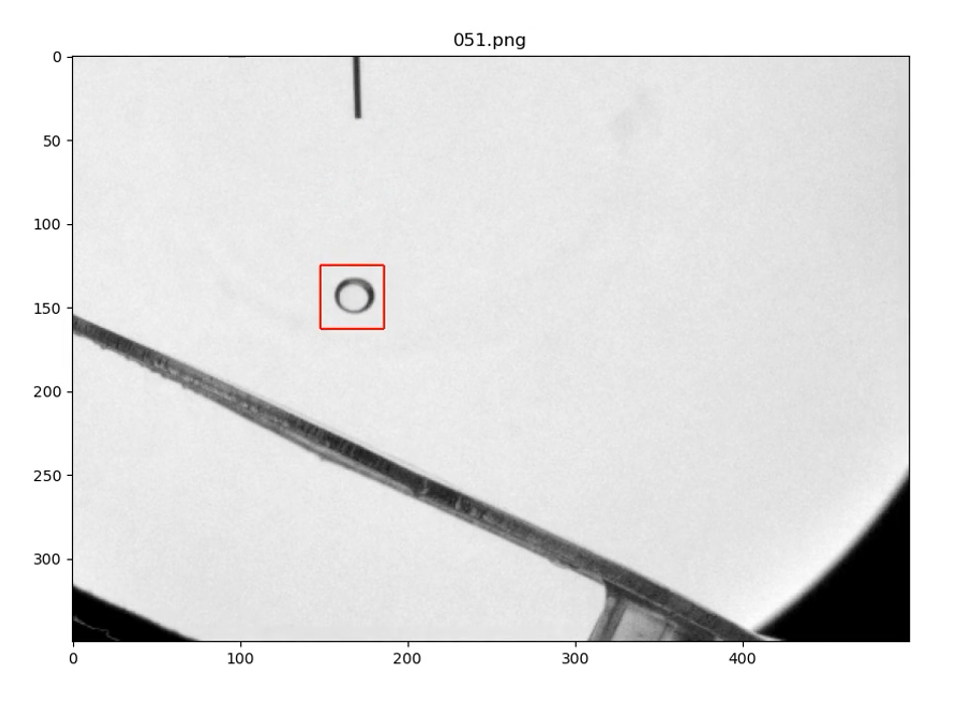
\includegraphics[scale=0.35]{dc_poster.png}}{dynamic_cropping.mp4}\\
    \small
    Of course, we still need to provide the crop coordiantes for a couple of frames. Even after this, the method gives results for just about 140 images out of 171.
\end{frame}
\begin{frame}
    \frametitle{Problems With The Main Method}
    \section{Problems With The Main Method}
    Here are some sample images and their center determined using the dynamic cropping method.\\
    \begin{figure}
        \centering
        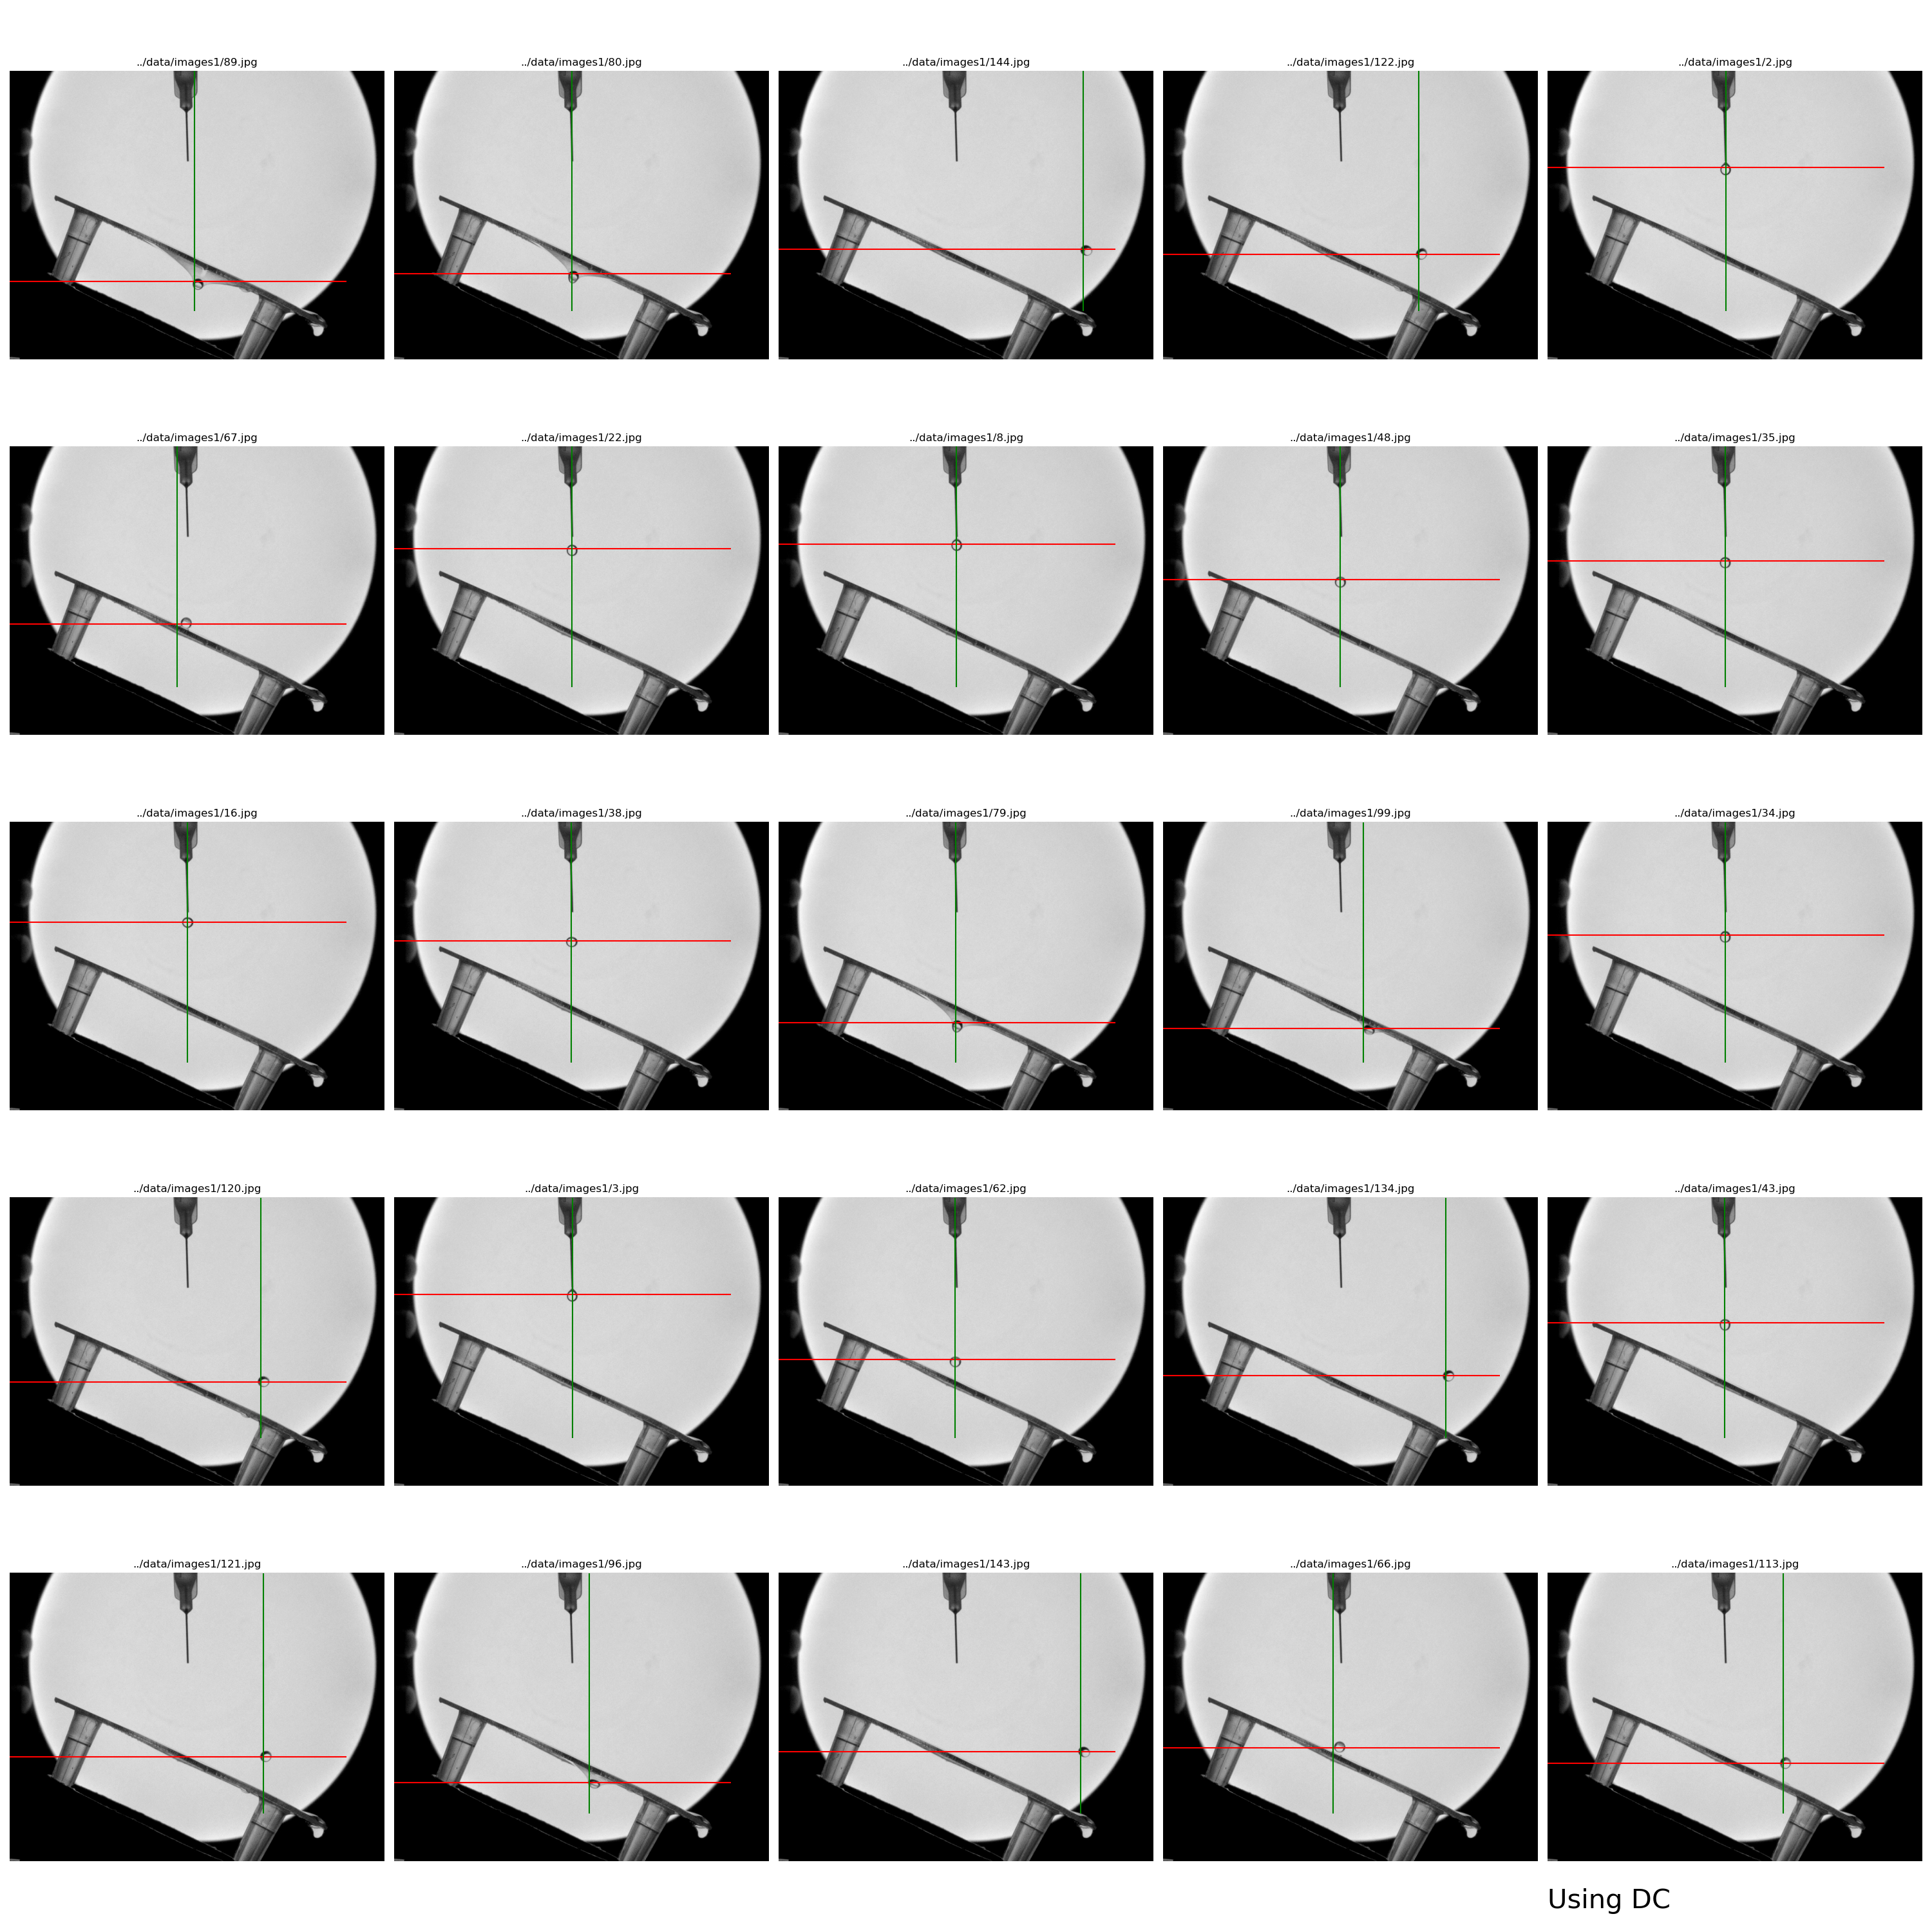
\includegraphics[scale=0.10]{using_dc.png}
    \end{figure}
\end{frame}
\begin{frame}
    \frametitle{More Robust Methods}
    \section{More Robust Methods}
    \Large \textbf{Subtracting The Background}\\
    \small
    We saw that the dynamic cropping method is not robust enough. The problem arises because the needle and the thin film in the image acts as noise which our method fails to detect. To overcome this problem we subtracted the image in consideration with a reference image.\\
    \onslide<2->
    \begin{figure}
        \centering
        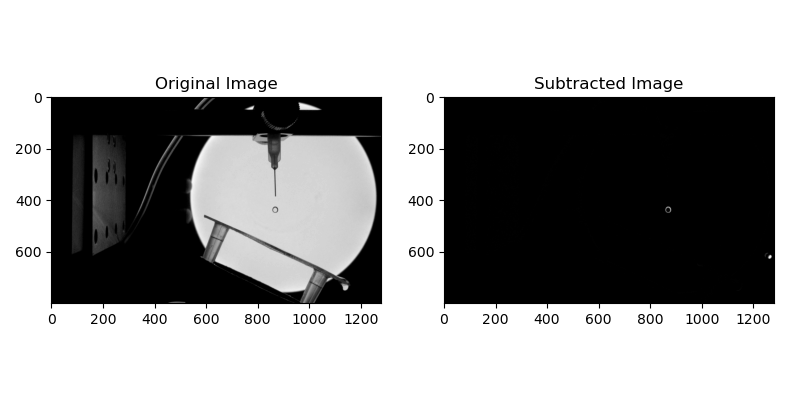
\includegraphics[scale=0.4]{subtracted.png}
        \caption[]{Original and Subtracted Image}
    \end{figure}
\end{frame}
\begin{frame}
    \frametitle{Subtracting The Background}
    Here is the reference image we used.\\
    \begin{figure}
        \centering
        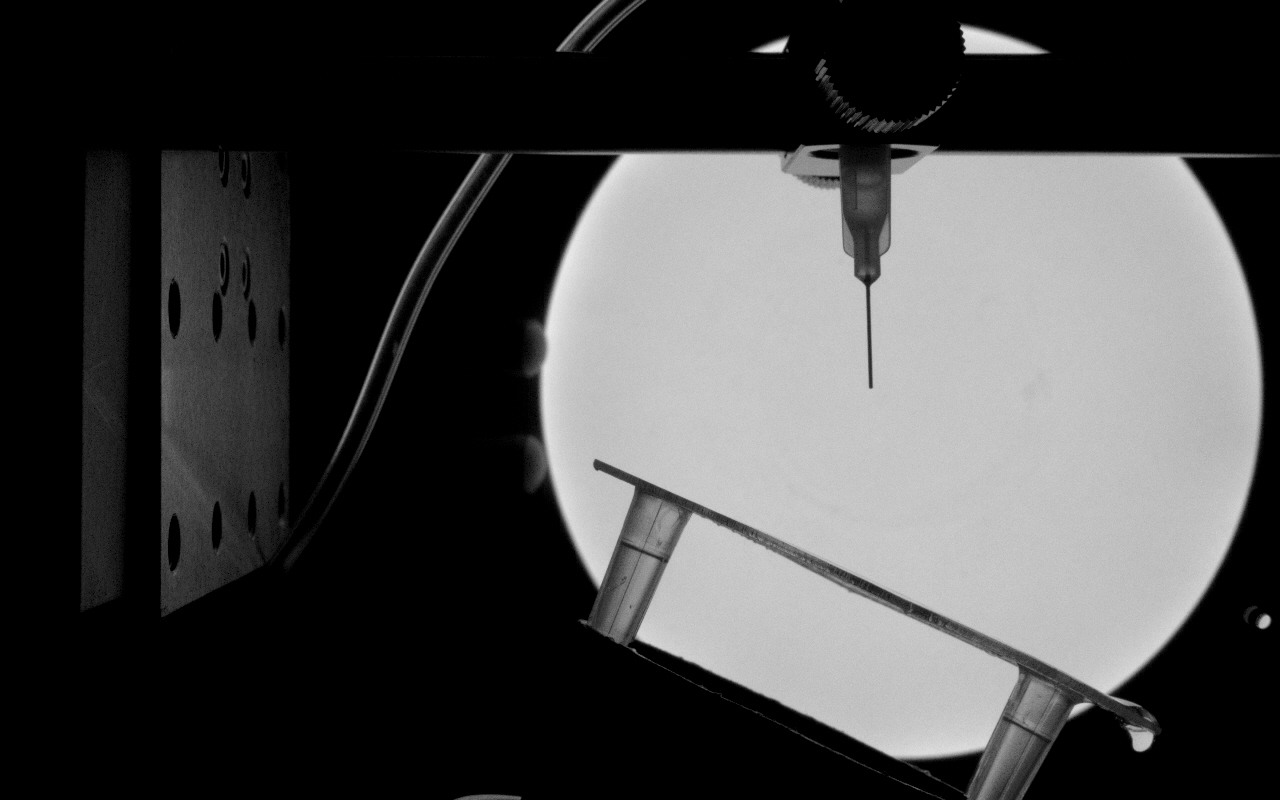
\includegraphics[scale=4]{ref_image.jpg}
        \caption[]{The Reference Image}
    \end{figure}
\end{frame}
\begin{frame}
    \frametitle{Subtracting the Background}
    \section{Subtracting the Background}
    \begin{itemize}
        \item <1->  As we can see, after subtracting from a reference image, the final image does not contain any background noise, just the drop. This means that the previous method should work very well.
        \item <2-> This was the case. This modification results in a better result. We were able to extract the center of more images (over 160 out of 172 images). Furthermore, the center extracted were more "accurate". The next slide shows some of the sample images with their center determined using the modified method.
    \end{itemize}
\end{frame}
\begin{frame}
    \begin{figure}
        \centering
        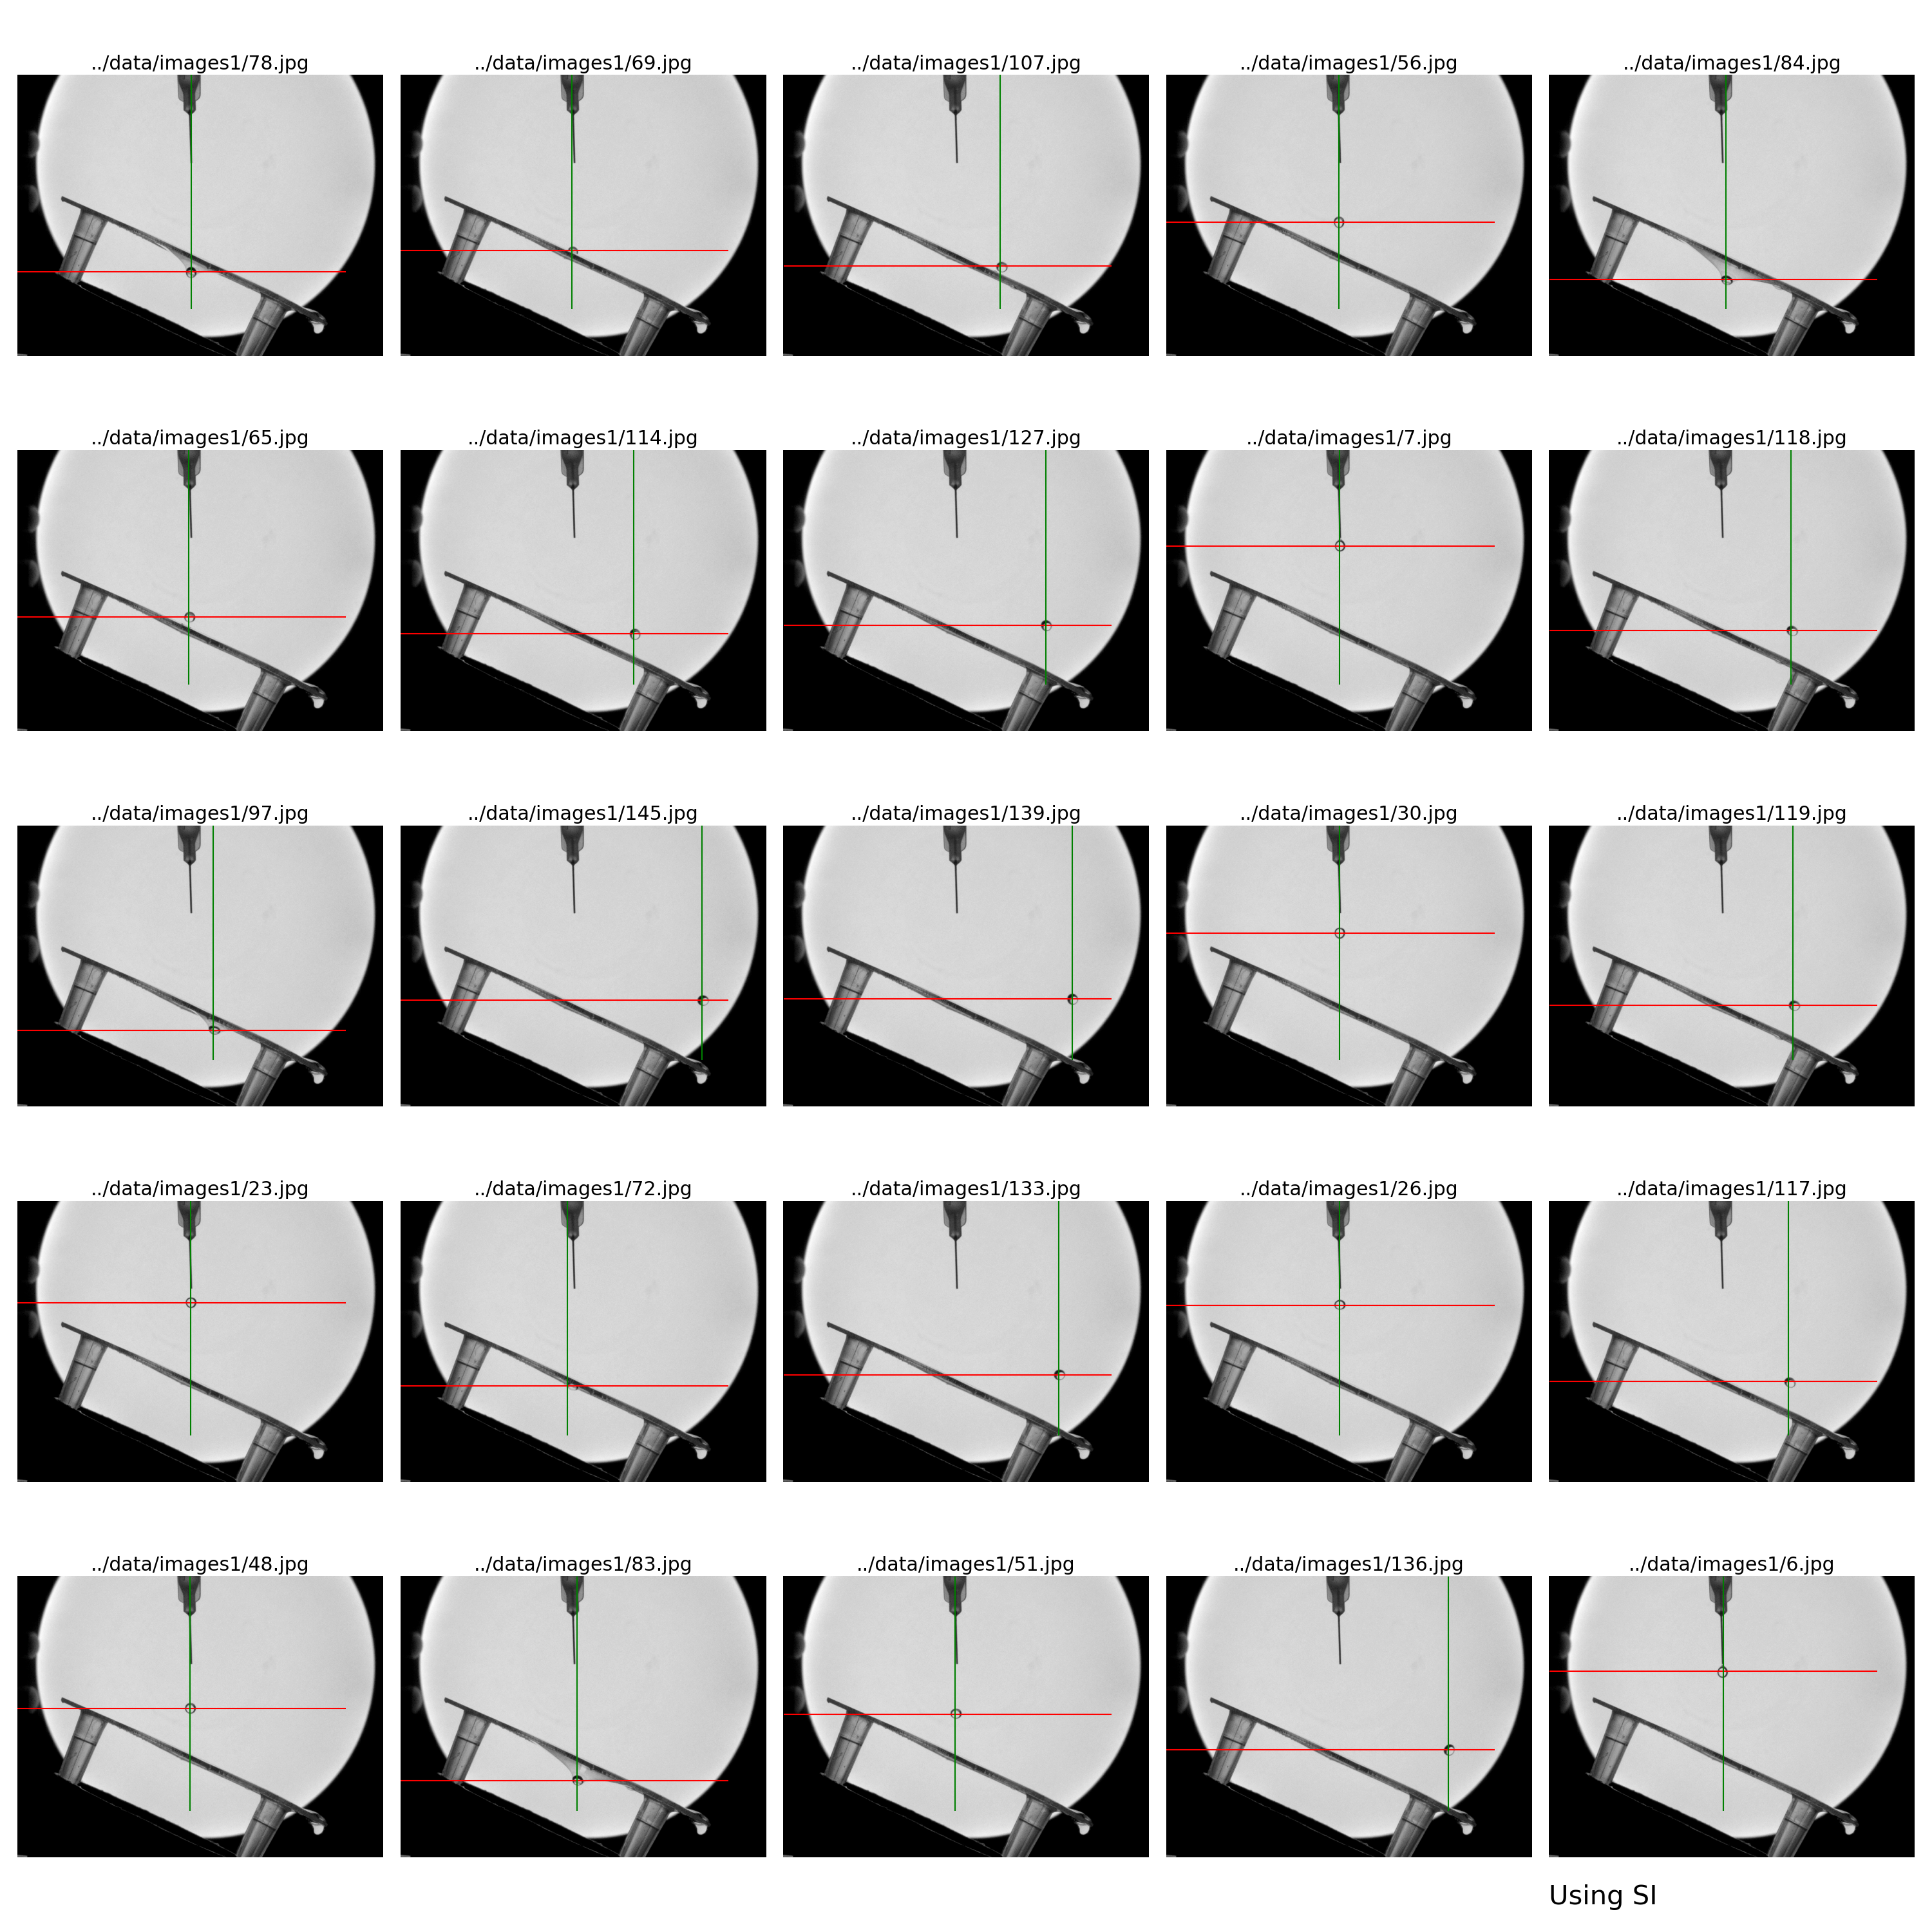
\includegraphics[scale=0.10]{using_si.png}
        \caption{Sample Images with Their Center Determined Using the Modified Method}
    \end{figure}
\end{frame}
\begin{frame}
    \frametitle{Fitting an Ellipse}
    \section{Fitting an Ellipse}
    \begin{enumerate}
        \item <1-> \textbf{Motivation}\\
              If we see the animation of the drop falling, we'll notice that the drop is oscillating and rotating. We wanted to see whether we can catch this rotation using some method. This was one of the main reasons why we decided to use the ellipse fitting method. Another reason was to further increase the accuracy of the center extracted.
        \item <2-> \textbf{Determining the Coordiantes}\\
              First step was to determine the coordinates of all the points which form the 'circumference' of the drop. This was determined by looping through the rows and columns and finding all the balck pixels, which are the points on the circumference of the drop.
    \end{enumerate}
\end{frame}
\begin{frame}
    \frametitle{Fitting an Ellipse}
    Here is an image showing how the points on the circumference are determined.\\
    \begin{figure}
        \centering
        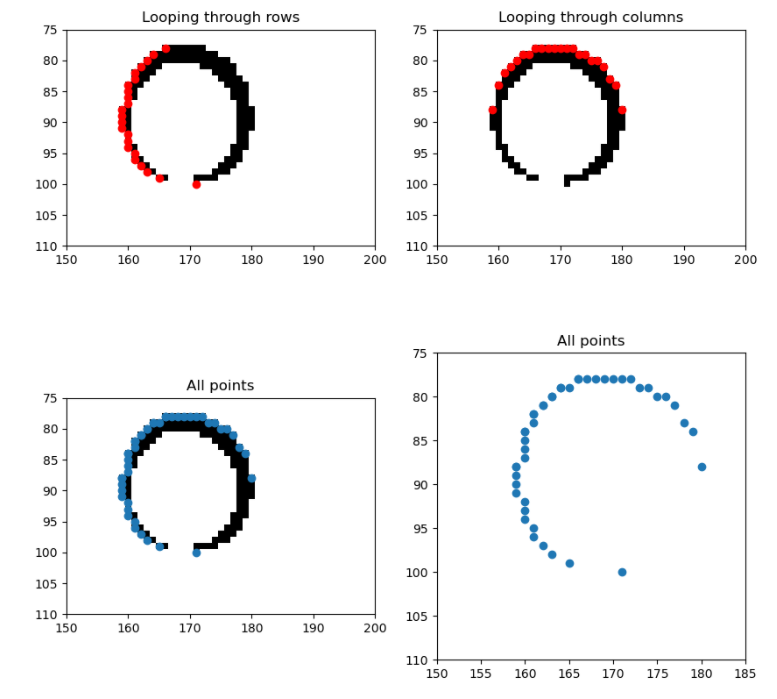
\includegraphics[scale=0.5]{all_points.png}
        \caption[]{Points on the Circumference of the Drop}
    \end{figure}
\end{frame}
\begin{frame}
    \frametitle{Fitting an Ellipse}
    \begin{columns}
        \column{0.5\textwidth}
        Once we have the coordiantes of all the points, we used the \textcolor{blue}{EllipseModel} class from the \textcolor{blue}{skimage} library to fit an ellipse to the points. The class fits an ellipse and return the parameters of the ellipse:
        \begin{itemize}
            \item The coordiantes of the center
            \item the semi major and minor axes
            \item The angle the major axis of the ellipse makes with the x-axis
        \end{itemize}
        \pause
        \column{0.5\textwidth}
        \begin{figure}
            \centering
            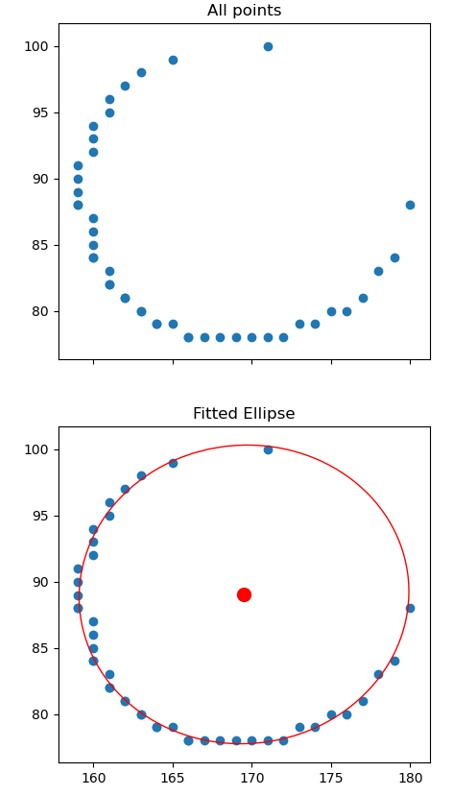
\includegraphics[scale=0.5]{ellipse_fit.png}
            \caption[]{Fitting an Ellipse}
        \end{figure}
    \end{columns}
\end{frame}
\begin{frame}
    \frametitle{Fitting an Ellipse}
    \small
    Though we were not able to infer the rotation of the drop, this method works better than the previous methods; in a sense that the center determined using this are more accurate. Here are some samples.
    \begin{figure}
        \centering
        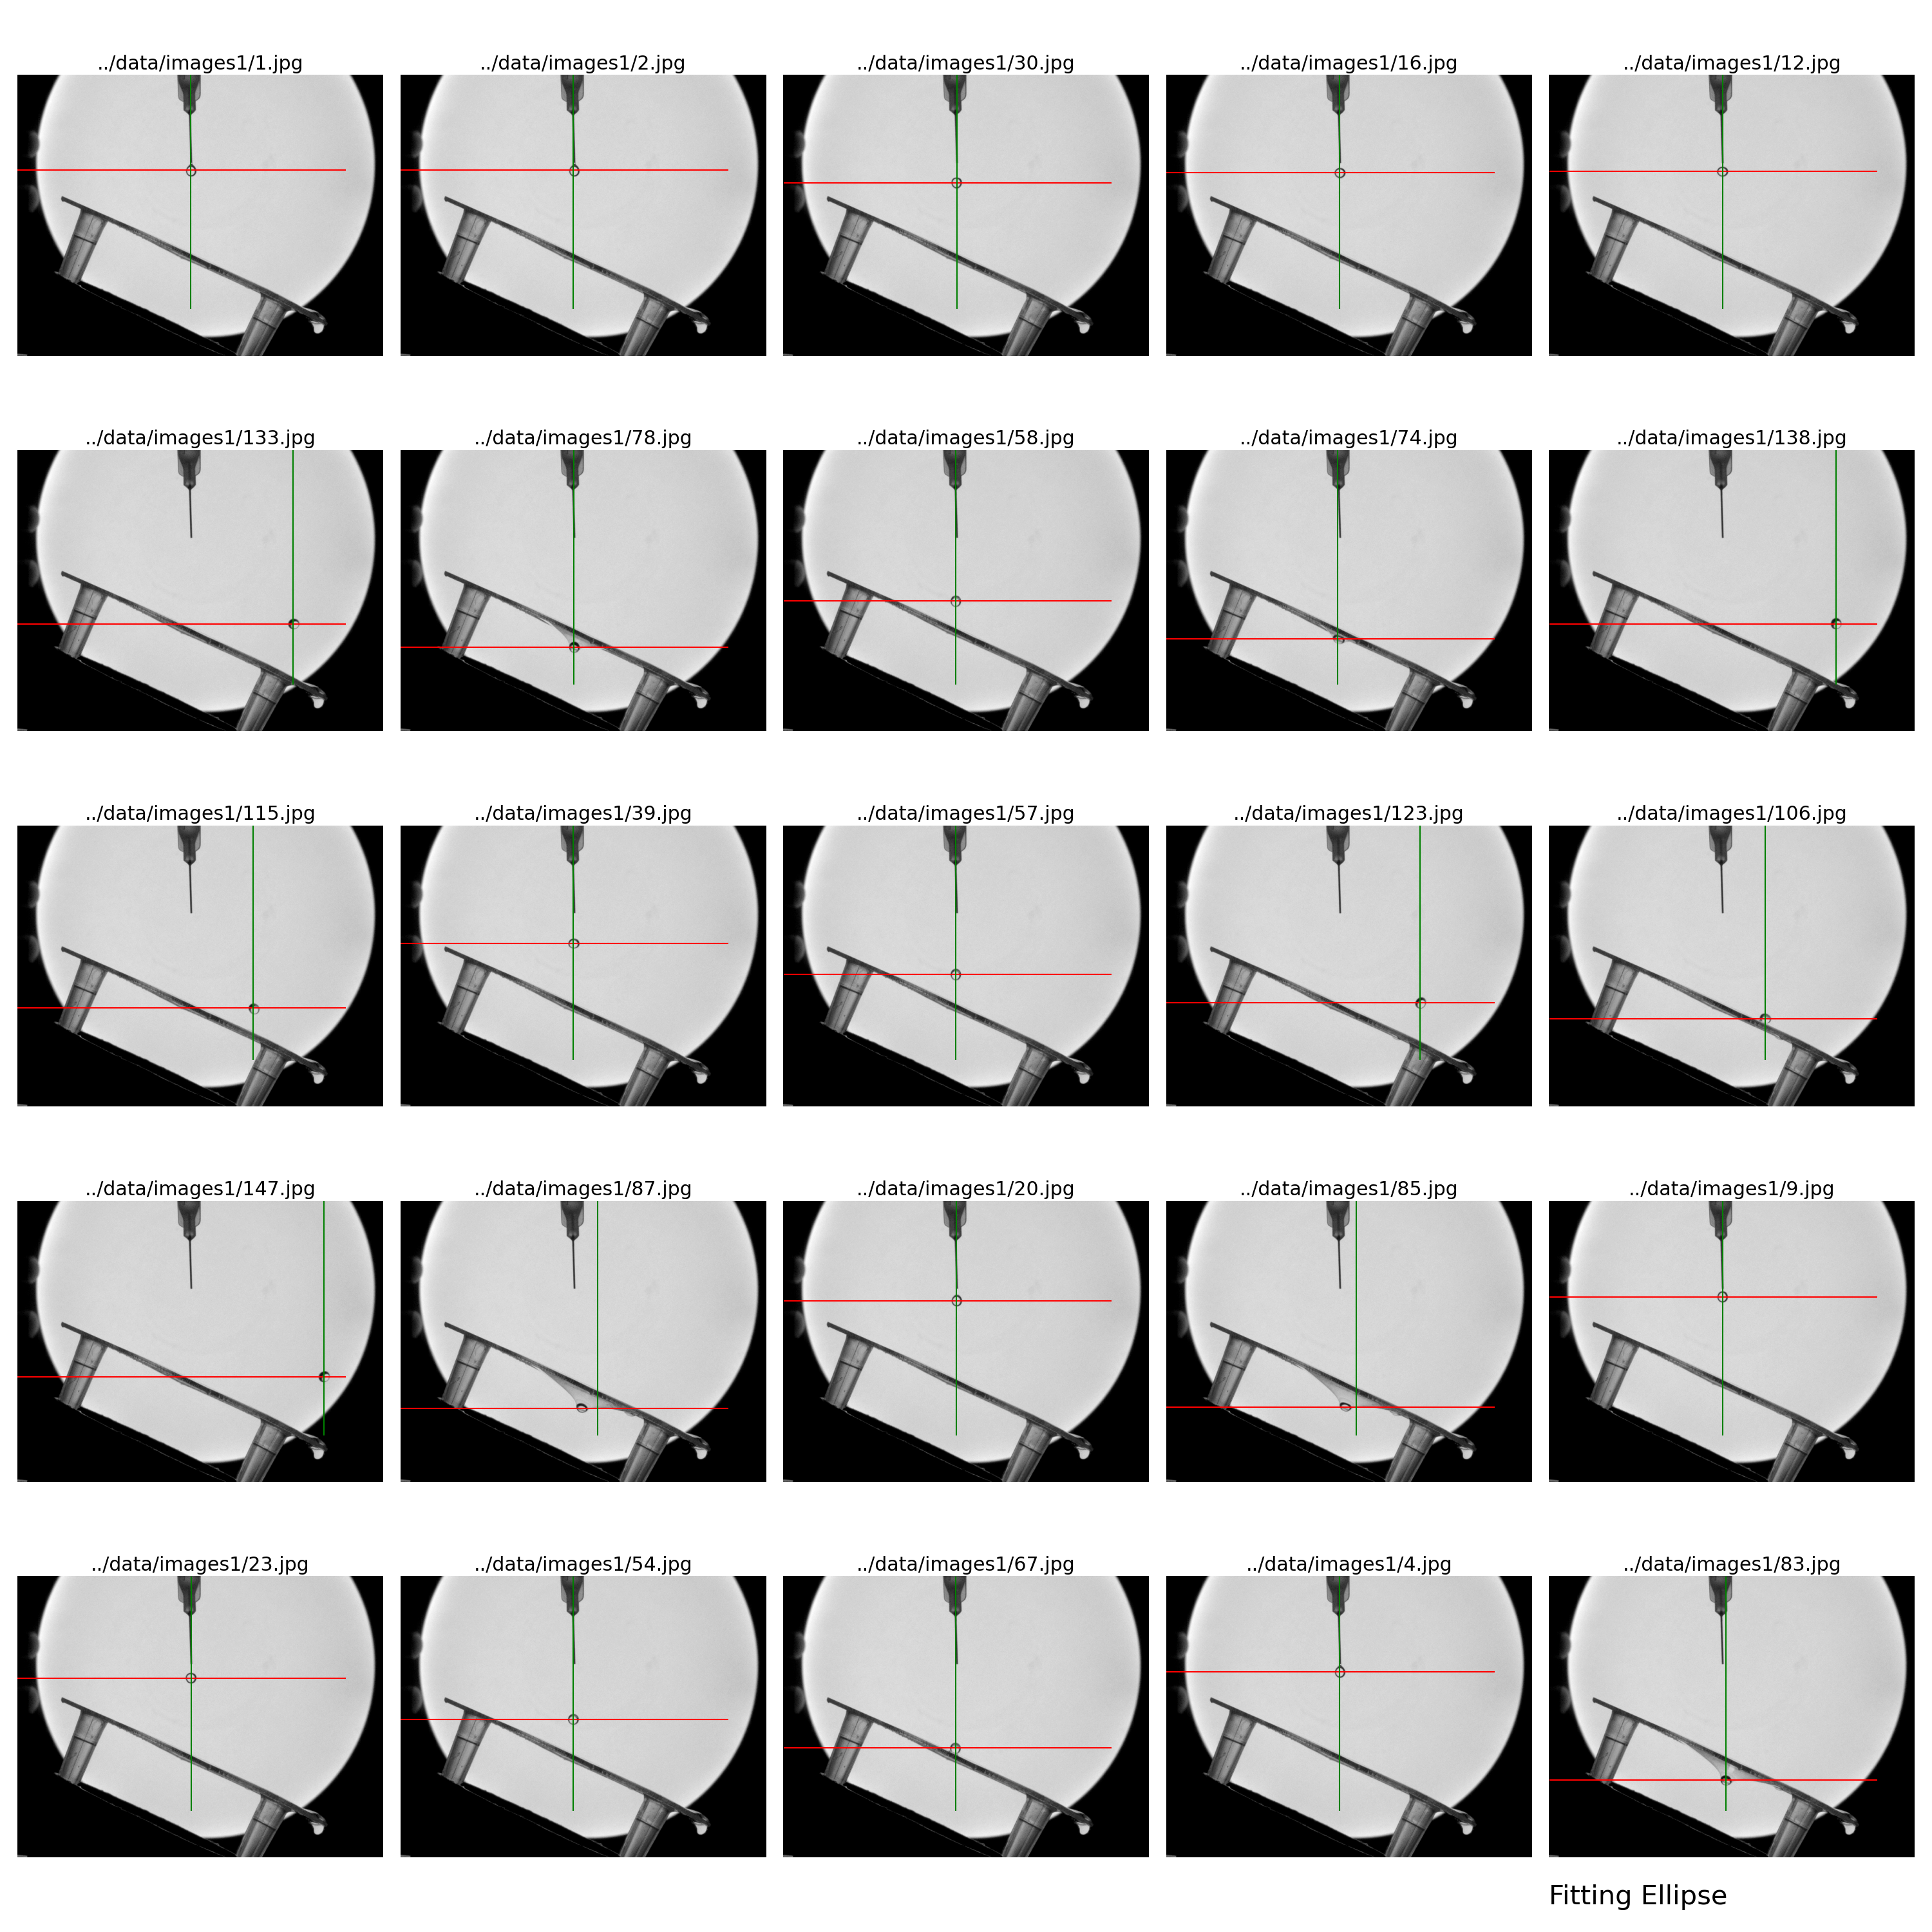
\includegraphics[scale=0.07]{using_ap.png}
        \caption[]{Sample Images by fitting an Ellipse}
    \end{figure}
\end{frame}
\begin{frame}
    \frametitle{Preliminary Analysis}
    \section{Preliminary Analysis}
    \onslide<1->
    Though our main focus till now has been to extract the coordiantes of the center of the drop with more and more accuracy, we also did some preliminary analysis on the extracted data, mainly to determine whether our method is working or not and to compare the different approaches we took.\\
    \onslide<2->
    So, we made some plots. We plotted \(x, y, v_x, v_y, r_1, r_2\) with time. We also plotted \(x \text{ vs } y, v_x \text{ vs } v_y, r_1 \text{ vs } r_2\). However, the most illuminating plots are those involving x and y.\\
    Next few silde will show the plots of x and y with time as well as for x with y. The plots are made using "raw data", that is, we did not make any smoothing or any other processing.\\
    We are working on some smoothing techniques. But it is work in progress.
\end{frame}
\begin{frame}
    \frametitle{Preliminary Analysis}
    \begin{figure}
        \centering
        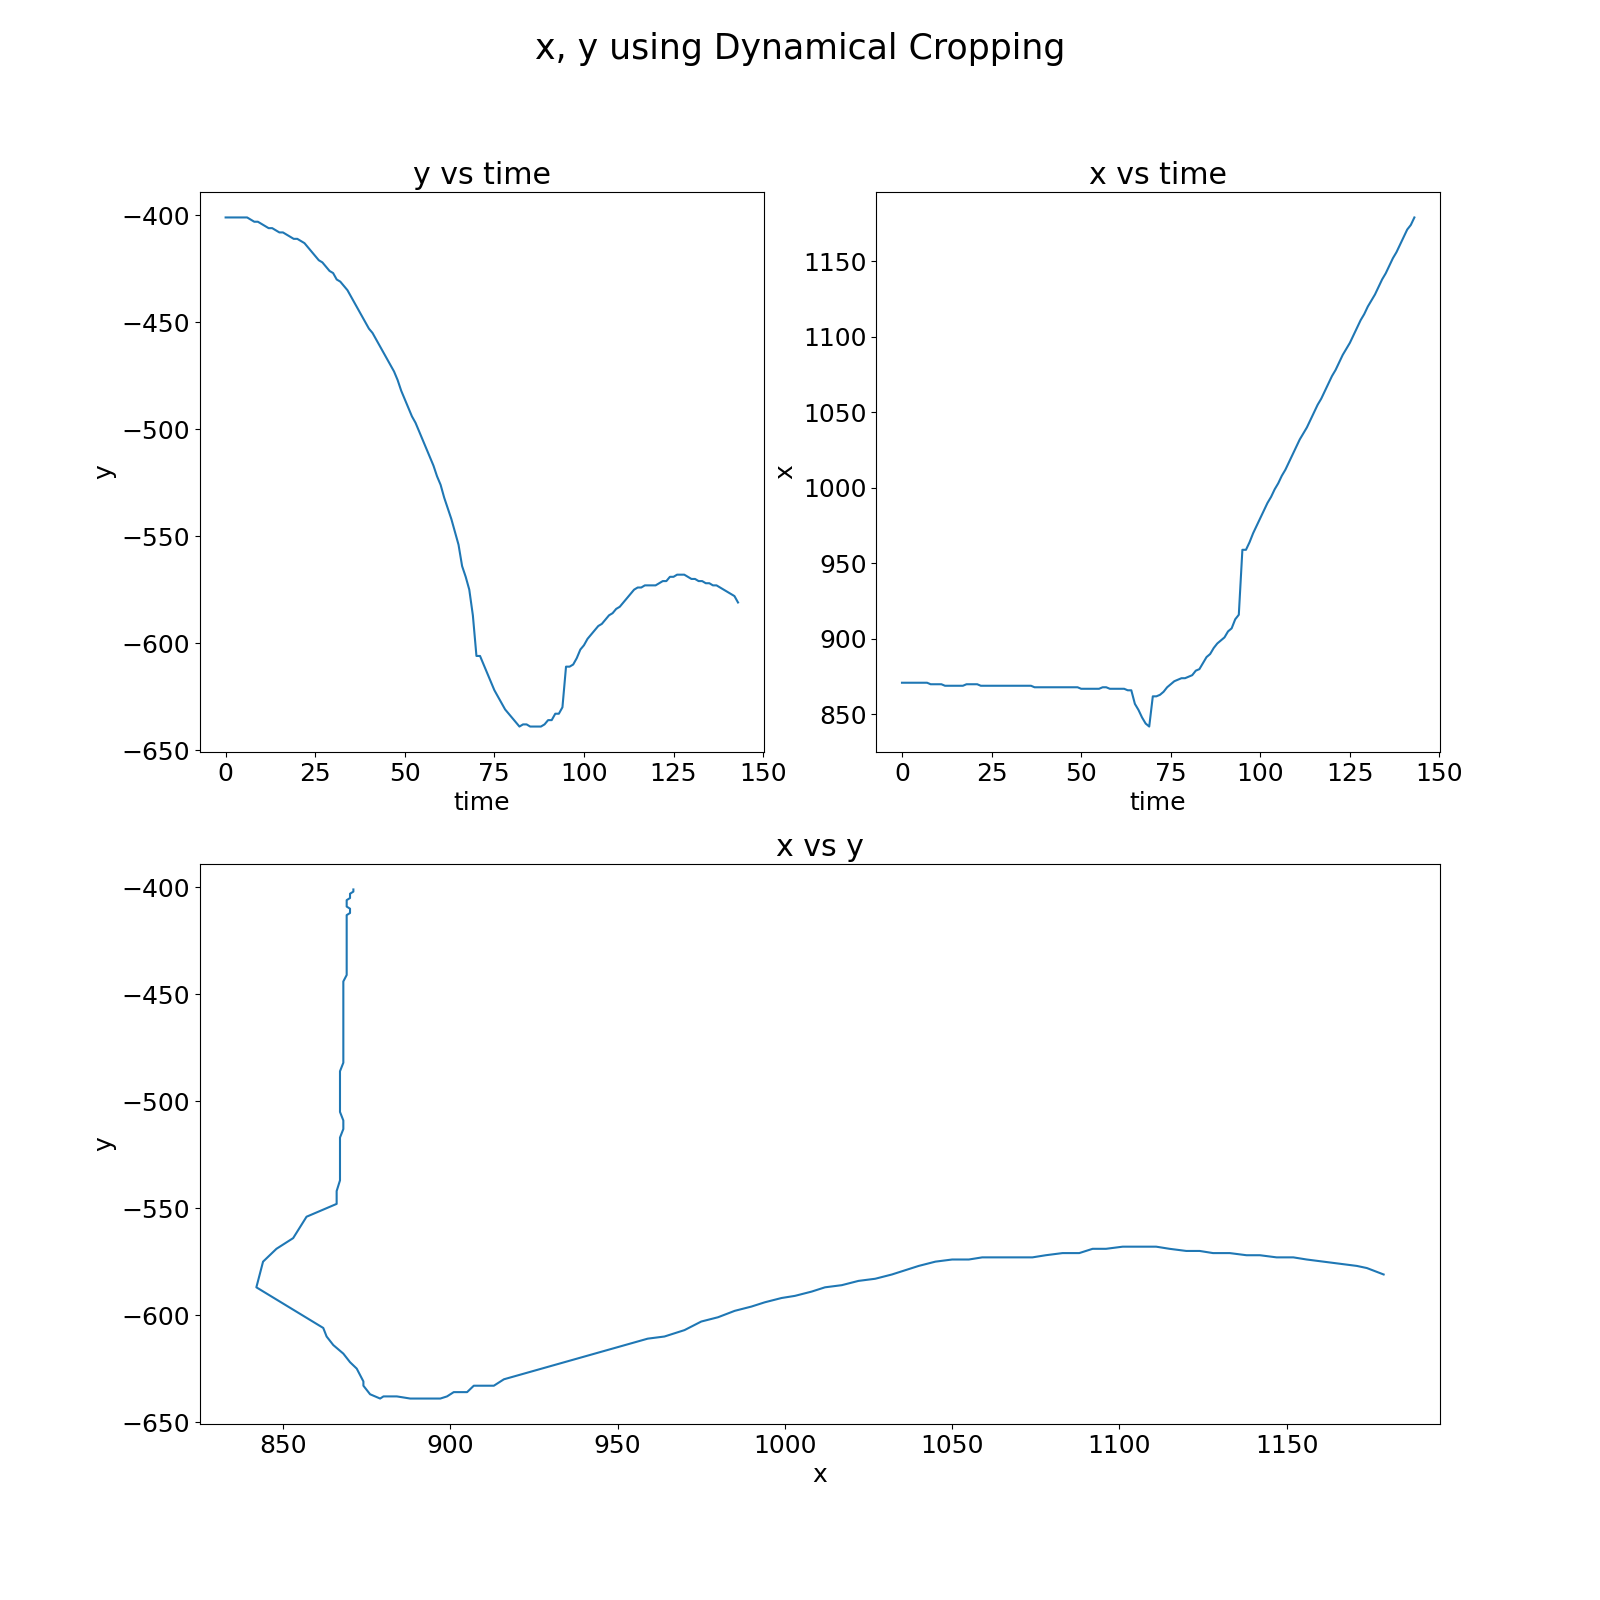
\includegraphics[scale=0.2]{x_y_using_dc.png}
        % \caption[]{Dynamic Cropping}
    \end{figure}
\end{frame}
\begin{frame}
    \frametitle{Preliminary Analysis}
    \begin{figure}
        \centering
        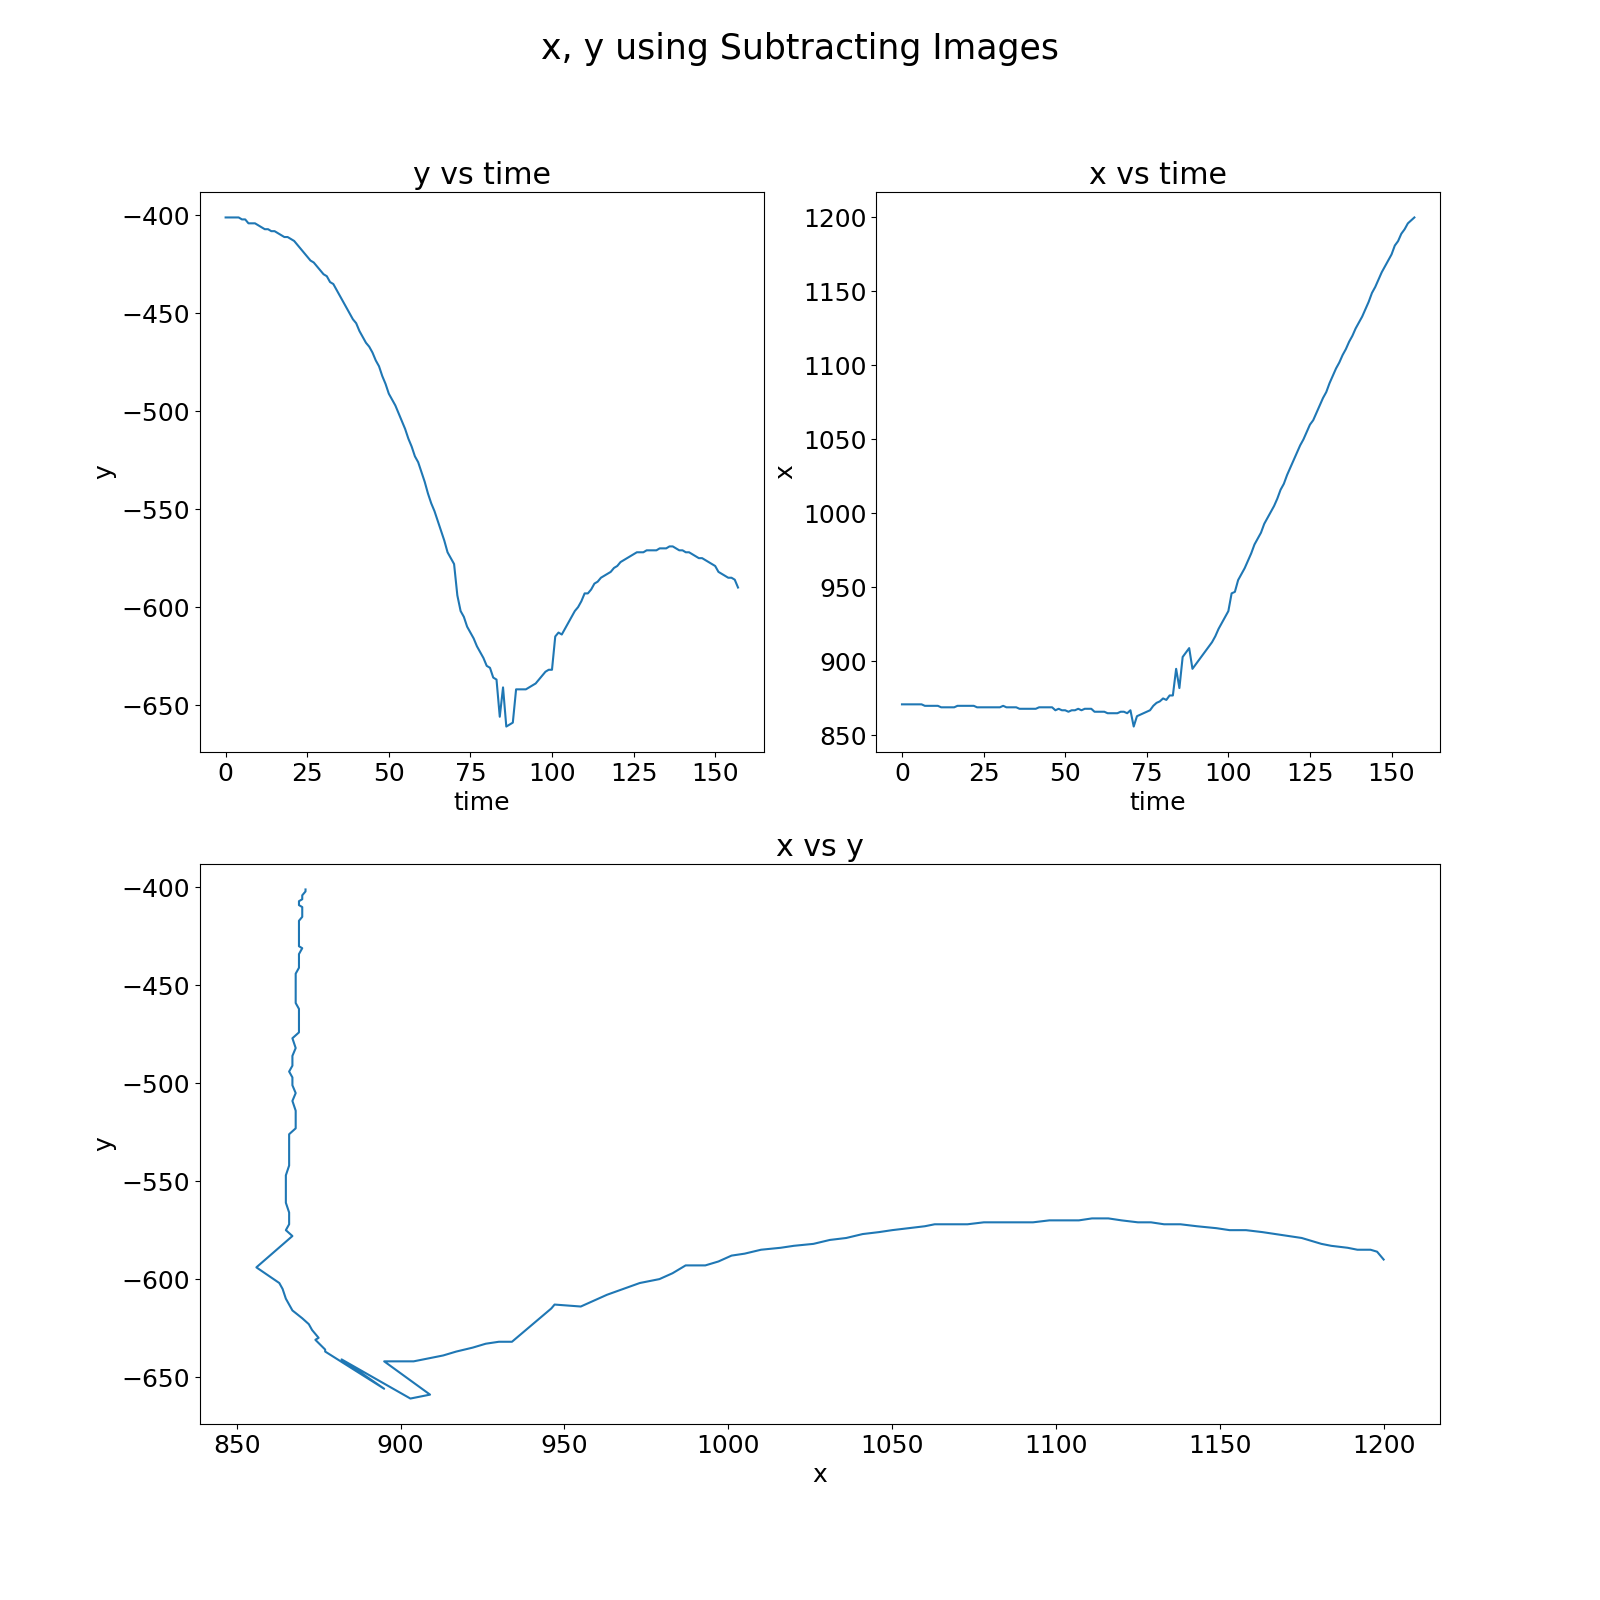
\includegraphics[scale=0.2]{x_y_using_si.png}
        % \caption[]{Subtracting Images}
    \end{figure}
\end{frame}
\begin{frame}
    \frametitle{Preliminary Analysis}
    \begin{figure}
        \centering
        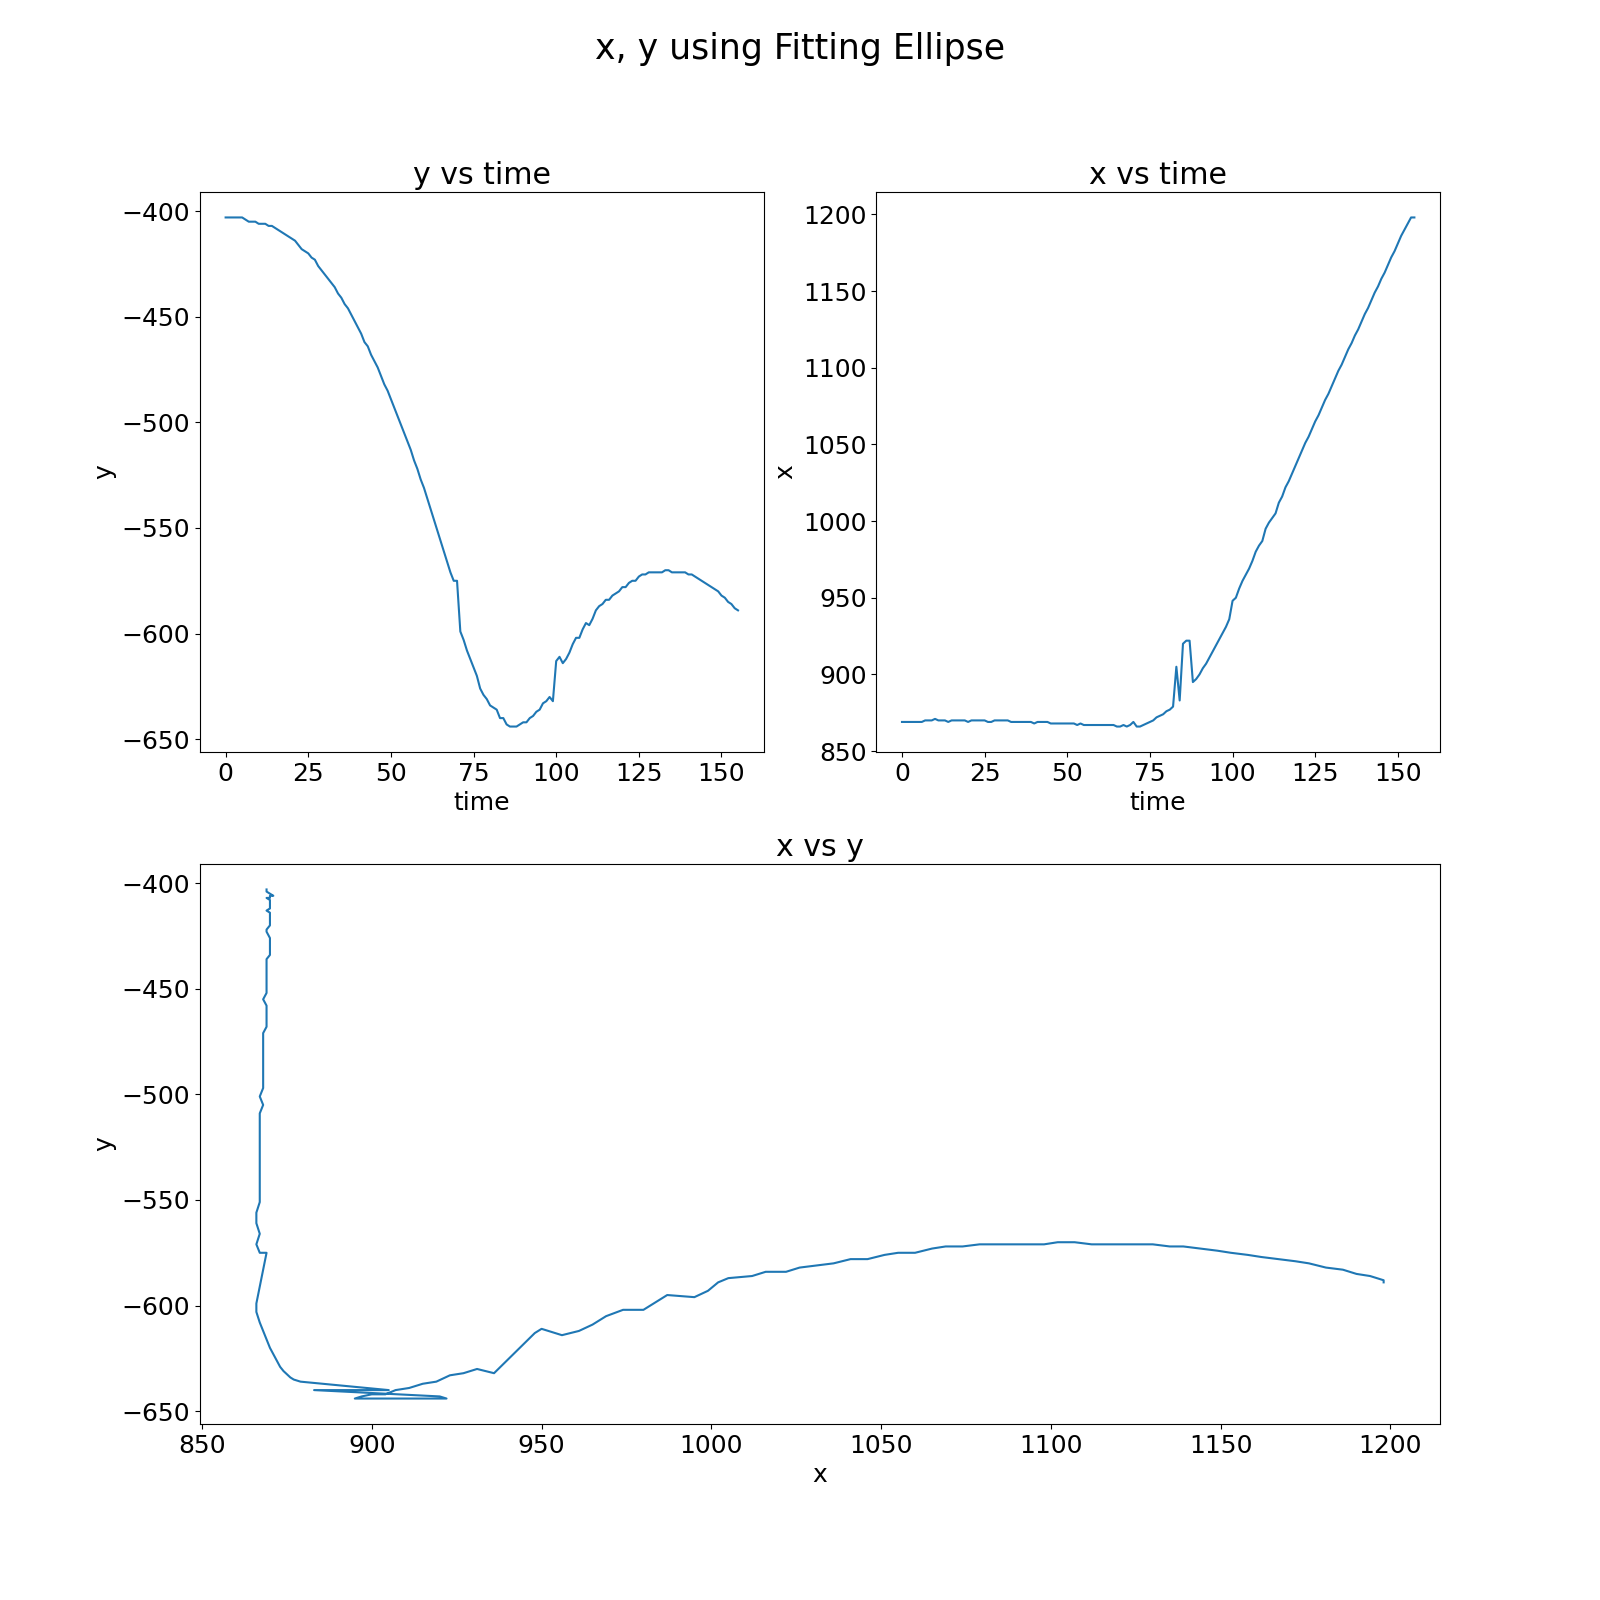
\includegraphics[scale=0.2]{x_y_using_ap.png}
        % \caption[]{Fitting an Ellipse}
    \end{figure}
\end{frame}
\begin{frame}
    \frametitle{What Next?}
    \section{What Next?}
    \begin{enumerate}
        \item <1-> \textbf{Smoothing}\\
              We are working on some smoothing techniques, like taking moving averages or using convolution.
        \item <2-> \textbf{Increasing Accuracy}\\
              Though fitting an ellipse is working very good, we are thinking of some ways to increase its accuracy even more. The main techniques, we are trying to implement are:
              \begin{itemize}
                  \item Using grayscale image instead of binary image
                  \item Plotting intensity vs time and using it to determine the coordinates
              \end{itemize}
    \end{enumerate}
\end{frame}
\end{document}